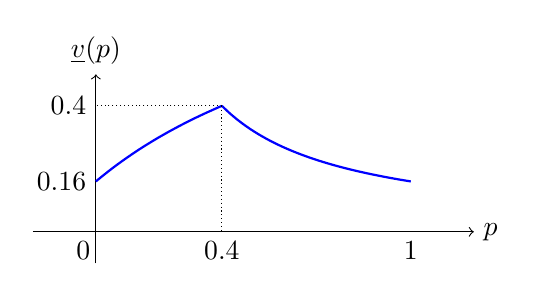
\begin{tikzpicture}[scale=4]
\draw[->] (-0.2, 0) -- (1.2, 0) node[right] {$p$};
\draw[->] (0, -0.1) -- (0, 0.5) node[above] {$\underline{v}(p)$};
\draw[domain=0:0.4, smooth, thick, variable=\x, blue] plot ({\x}, {(0.16 + \x)/(1 + \x)});
\draw[domain=0.4:1, smooth, thick, variable=\x, blue] plot ({\x}, {0.16/\x});
\draw[densely dotted] (0.4, 0.4) -- (0.4, 0);
\draw[densely dotted] (0.4, 0.4) -- (0, 0.4);
\node at (-0.04,0) [below] {$0$};
\node at (0.4,0) [below] {$0.4$};
\node at (1,0) [below] {$1$};
\node at (0,0.16) [left] {$0.16$};
\node at (0,0.4) [left] {$0.4$};
\end{tikzpicture}